\documentclass[letterpaper,11pt]{article}

% --- PAQUETES DE IDIOMA
\usepackage[spanish,mexico]{babel}
\usepackage[utf8]{inputenc}
\usepackage{csquotes}
\usepackage{iftex}

\usepackage{pdfpages}

% --- PAQUETES MATEMÁTICOS --
\usepackage{amsmath}
\usepackage{cancel}
\usepackage{mathrsfs}

% --- PAQUETES GRÁFICOS Y DE DISEÑO ---
\usepackage{graphicx}
\usepackage{float}
\usepackage{placeins}
\usepackage{subcaption}
\usepackage[table]{xcolor}
\usepackage{makecell}
\usepackage{array}
\usepackage{tikz}
\usetikzlibrary{shapes.geometric, shapes.multipart, positioning, arrows.meta, calc, shadows, decorations.pathreplacing,babel}

% --- LISTAS ---
\usepackage{enumitem}

% --- PAQUETES DE CÓDIGO ---
\usepackage{listings}
% Configuración del estilo de listings
\definecolor{codebg}{rgb}{0.95,0.95,0.95}   
\definecolor{keyword}{rgb}{0.0,0.2,0.6}     
\definecolor{comment}{rgb}{0.25,0.5,0.35}   
\definecolor{string}{rgb}{0.6,0.0,0.0}      
\definecolor{number}{rgb}{0.5,0.0,0.5}      
\definecolor{codegray}{rgb}{0.5,0.5,0.5}
\definecolor{codepurple}{rgb}{0.58,0,0.82}
\definecolor{backcolour}{rgb}{0.95,0.95,0.95}

\lstset{
  backgroundcolor=\color{backcolour},
  basicstyle=\ttfamily\small,
  keywordstyle=\color{blue}\bfseries,
  stringstyle=\color{codepurple},
  commentstyle=\color{codegray}\itshape,
  numbers=left,
  numberstyle=\tiny\color{codegray},
  frame=single,
  rulecolor=\color{black},
  breaklines=true,
  tabsize=4,
  showstringspaces=false,
  literate={á}{{\'a}}1
           {é}{{\'e}}1
           {í}{{\'i}}1
           {ó}{{\'o}}1
           {ú}{{\'u}}1
           {Á}{{\'A}}1
           {É}{{\'E}}1
           {Í}{{\'I}}1
           {Ó}{{\'O}}1
           {Ú}{{\'U}}1
           {ñ}{{\~n}}1
           {Ñ}{{\~N}}1
           {¿}{{\textquestiondown}}1
           {¡}{{\textexclamdown}}1
}

% Estilo para código en C
\lstdefinestyle{cstyle}{
  language=C,
  backgroundcolor=\color{backcolour},
  basicstyle=\ttfamily\small,
  keywordstyle=\color{blue}\bfseries,
    keywordstyle=[2]\color{yellow!70!orange}\bfseries,
    morekeywords=[2]{MPI_Init,MPI_Comm_size,MPI_Comm_rank,MPI_Send,MPI_Recv,MPI_Scatter,MPI_Gather,MPI_Bcast,MPI_Reduce,MPI_Finalize},
    emph={printf},
    emphstyle=\color{blue}\bfseries,
  stringstyle=\color{codepurple},
  commentstyle=\color{codegray}\itshape,
  numbers=left,
  numberstyle=\tiny\color{codegray},
  frame=single,
  rulecolor=\color{black},
  breaklines=true,
  tabsize=4,
  showstringspaces=false
}

% Definición del lenguaje Python para listings
\lstdefinelanguage[LAB]{Python}{
    morekeywords={False, None, True, and, as, assert, async, await, break,
                                class, continue, def, del, elif, else, except, finally,
                                for, from, global, if, import, in, is, lambda, nonlocal,
                                not, or, pass, raise, return, try, while, with, yield,
                                machine, Pin, PWM, ADC, Timer, sleep_ms, sleep_us},
    morecomment=[l]{\#},
    morestring=[b]",
    morestring=[b]',
    sensitive=true
}

% Estilo para salidas de consola/terminal
\lstdefinestyle{output}{
  backgroundcolor=\color{black!5},
  basicstyle=\ttfamily\footnotesize,
  numbers=none,
  frame=single,
  rulecolor=\color{black!30},
  breaklines=true,
  tabsize=4,
  showstringspaces=false,
  xleftmargin=0.5cm,
  xrightmargin=0.5cm
}

% --- ESTILOS PARA DIAGRAMAS DE FLUJO (TIKZ) ---
\tikzset{
  startstop/.style={rectangle, rounded corners, minimum width=3cm, minimum height=1cm,text centered, draw=black, fill=red!30},
  process/.style={rectangle, minimum width=3cm, minimum height=1cm, text centered, draw=black, fill=orange!30},
  decision/.style={diamond, aspect=2, minimum width=3cm, minimum height=1cm, text centered, draw=black, fill=green!30},
  io/.style={trapezium, trapezium left angle=70, trapezium right angle=110, minimum width=3cm, minimum height=1cm, text centered, draw=black, fill=blue!30},
  arrow/.style={thick,->,>=stealth}
}


\definecolor{azulresultado}{HTML}{0072C6}
\definecolor{rojoacarreo}{HTML}{FF0000}

% --- RUTAS DE IMÁGENES ---
\graphicspath{{img/}{portada_img/}}

\definecolor{armblue}{RGB}{0, 113, 188}

% --- ÍNDICE CON PUNTOS ---
\usepackage{tocloft}
\renewcommand{\cftsecleader}{\cftdotfill{\cftdotsep}}

% --- CONFIGURACIÓN DE PÁGINA (GEOMETRÍA) ---
\usepackage[
    left=25mm, 
    right=25mm,
    top=35mm,
    bottom=30mm,
    headheight=77pt, 
    papersize={21.59cm,27.94cm}
]{geometry}

% --- FORMATO DE TEXTO ---
\usepackage{setspace}
\onehalfspacing
\usepackage{parskip} 
\usepackage{lipsum}  

% --- VARIABLES GLOBALES ---
\newcommand{\materia}{}

% --- ENCABEZADOS Y PIES DE PÁGINA ---
\usepackage{fancyhdr}
\pagestyle{fancy}
\fancyhf{} 
\fancyhead[L]{
\includegraphics[height=1.5cm]{portada_img/der.png}}
\fancyhead[R]{
\includegraphics[height=1.5cm]{portada_img/izq.png}}
\fancyfoot[C]{\thepage} 
\renewcommand{\headrulewidth}{0.4pt} 
\renewcommand{\footrulewidth}{0pt}  

% --- BIBLIOGRAFÍA ---
\usepackage[backend=biber, style=apa, sortcites, url=true]{biblatex}
\addbibresource{referencias.bib}

% --- HIPERVÍNCULOS ---
\usepackage{hyperref}
\hypersetup{
    colorlinks=true,
    linkcolor=blue,
    citecolor=blue,
    filecolor=magenta,
    urlcolor=cyan
}

\begin{document}

\input{portada.tex}

\newpage
{\hypersetup{linkcolor=black}\tableofcontents}
\thispagestyle{empty}

\newpage

\setcounter{page}{1}
\singlespacing

\section{Actividad 1:}

\subsection{Comando fdisk:}

El comando fdisk en linux, es un comando que se coloca directamente en la terminal,
esto es para poder crear, eliminar, redimensionar, y administrar particiones de disco del propio sistema, no obstante 
tenemos que tener en cuenta que el comando fdisk en cuestion de usuarios con permisos, es un comando que solo puede ser ejecutado por el usuario root, 
esto es debido a que el comando fdisk tiene 
acceso a la tabla de particiones del disco duro, 
y si un usuario sin permisos de administrador lo ejecuta, 
este no tendra acceso a la tabla de particiones y por lo tanto no podra ejecutar el comando.

\subsection{Comando fdisk -l:}

Al agregar el parametro -l al mismo comando de fdisk, este nos mostrara un listado de todas las particiones que se encuentran en el disco duro,
ademas de que nos mostrara informacion adicional de cada particion, como lo es el tamaño de la particion, el tipo de particion, el sistema de archivos que tiene cada particion, y el estado de cada particion.

\subsection{Comando whoami:}

El comando whoami en linux, es un comando que se coloca directamente en la terminal, esto es para poder mostrar el nombre del usuario que esta actualmente logeado en el sistema.

\begin{figure}[H]
    \centering
    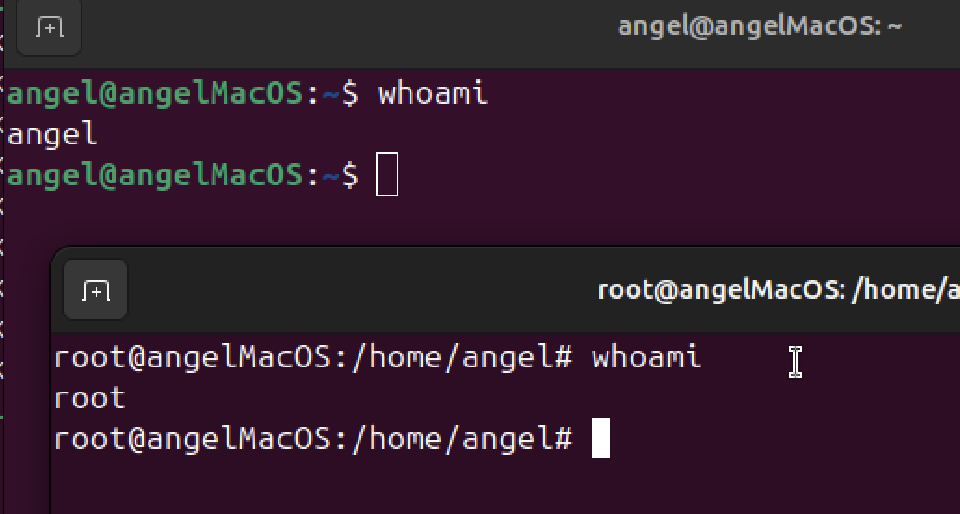
\includegraphics[width=0.7\textwidth]{image/image0.png}
    \caption{Ejecución del comando whoami.}
\end{figure}

\subsection{Ejecucion del comando fdisk -l:}

En el caso de este comando para el usuario no root, como se muestra en la imagen 
en todos los casos nos salen los permisos denegados, dejando en claro que este usuario no tiene 
el nivel acceso necesario.

\newpage

\begin{figure}[H]
    \centering
    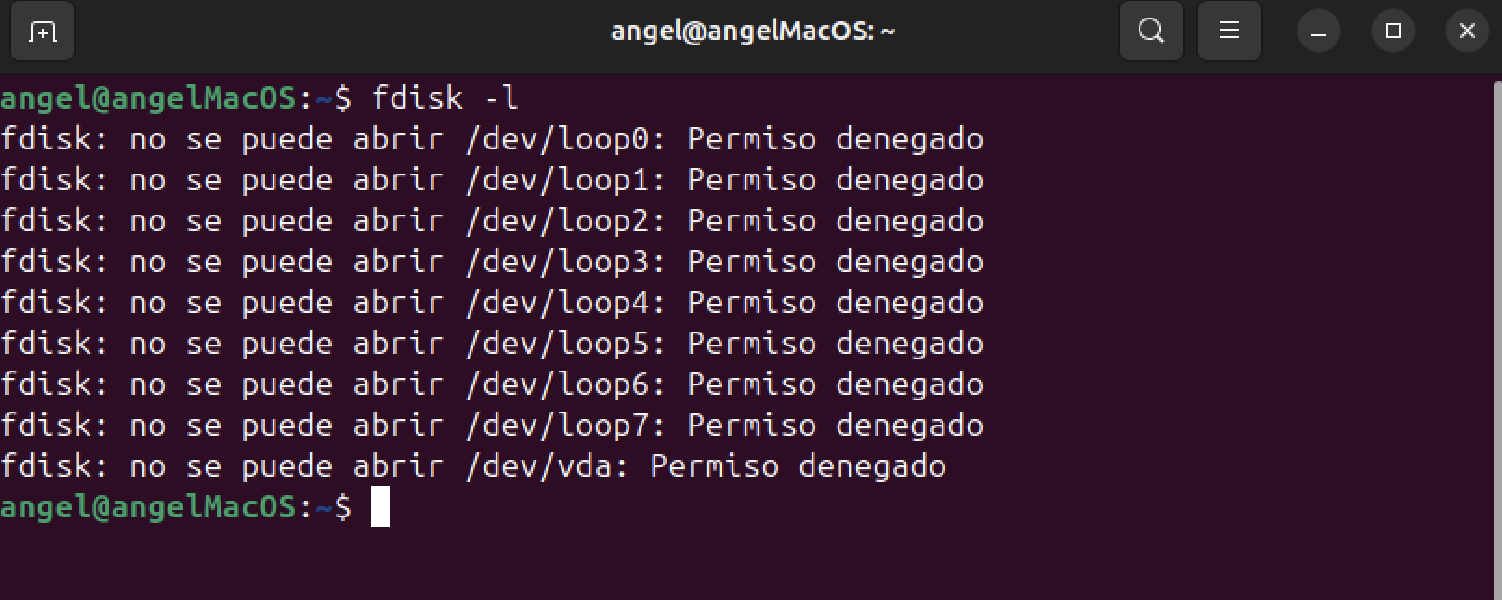
\includegraphics[width=0.7\textwidth]{image/image1.png}
    \caption{Ejecución del comando fdisk -l, para usuario no root.}
\end{figure}

En el caso del usurio root, se muestra como se deja ver las particiones del disco sin problema alguno:

\begin{figure}[H]
    \centering
    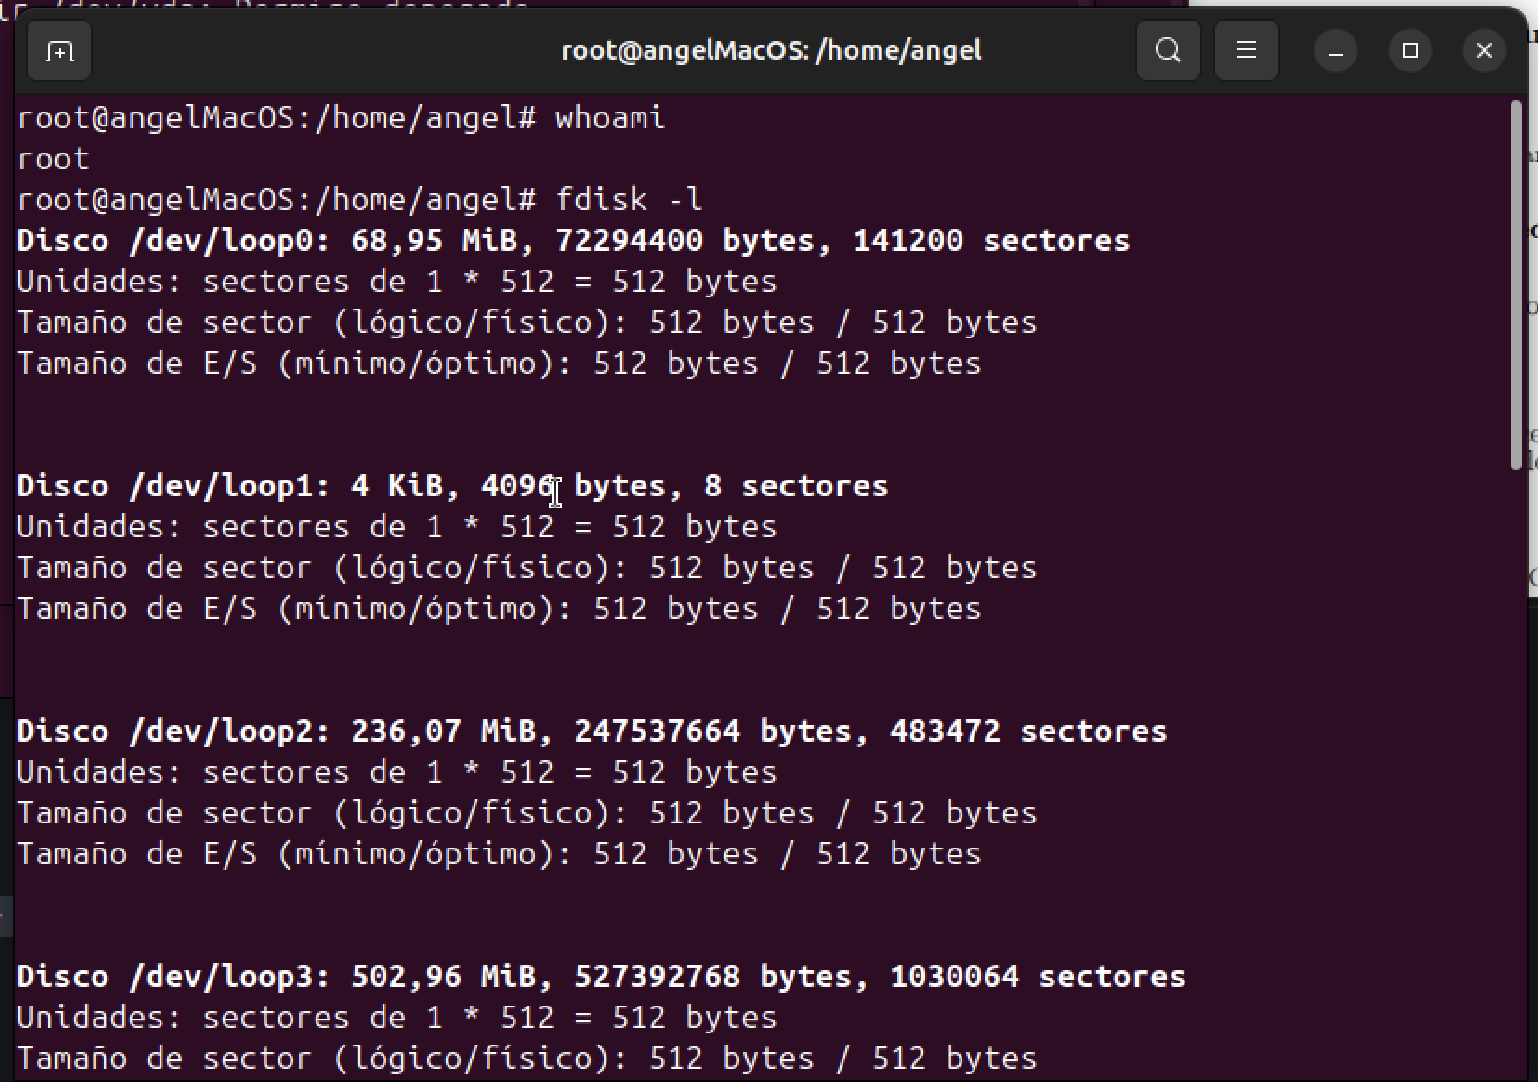
\includegraphics[width=0.7\textwidth]{image/image2.png}
    \caption{Ejecución del comando fdisk -l, para usuario root.}
\end{figure}

\subsection{Comando ls -l /sbin/fdisk:}

Para el caso de este comando ls -l /sbin/fdisk, se ejecuta si o si en la terminal 
del usuario root, esto es para poder ver los permisos que tiene el comando fdisk, y como se puede ver en la imagen, el comando fdisk tiene permisos de lectura, escritura y ejecucion para el usuario root, y permisos de lectura y ejecucion para el grupo y para los demas usuarios.
\newpage

\begin{figure}[H]
    \centering
    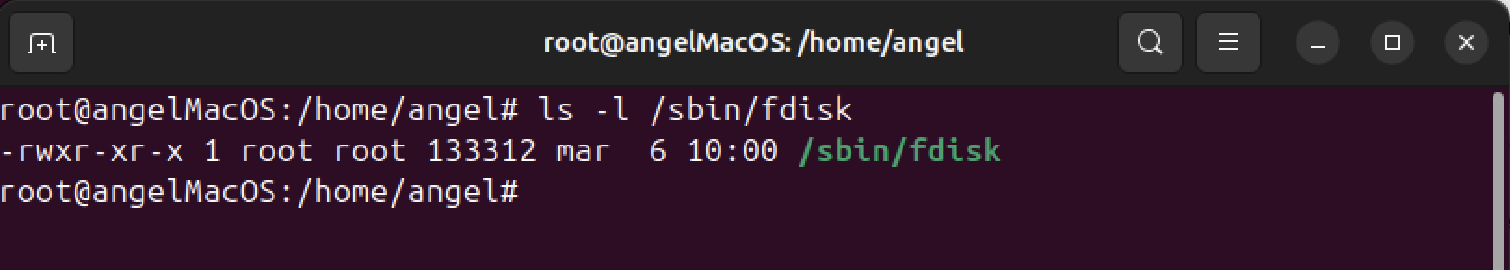
\includegraphics[width=0.7\textwidth]{image/image3.png}
    \caption{Ejecución del comando ls -l /sbin/fdisk, para usuario root.}
\end{figure}

\subsection{Comando chmod para activar el setuid:}

Para el caso de este comando, se tiene que colocar en la terminal el siguiente comando \texttt{chmod 4511 /sbin/fdisk}, esto 
para poder activar el setuid, esto es para que el comando fdisk pueda ser ejecutado por cualquier usuario, y este tenga los permisos del usuario root, esto es debido a que el comando fdisk tiene acceso a la tabla de particiones del disco duro, y si un usuario sin permisos de administrador lo ejecuta, este no tendra acceso a la tabla de particiones y por lo tanto no podra ejecutar el comando.

\begin{figure}[H]
    \centering
    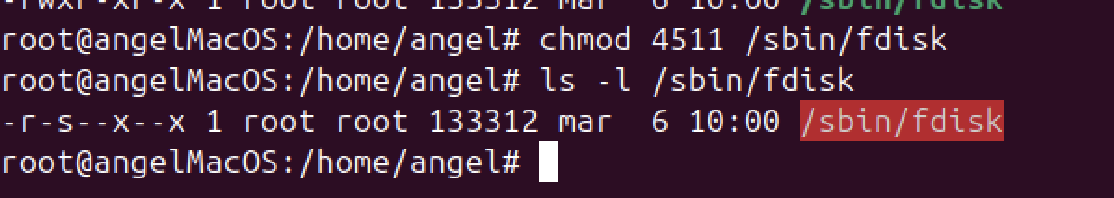
\includegraphics[width=0.7\textwidth]{image/image4.png}
    \caption{Ejecución del comando chmod para activar el setuid.}
  
\end{figure}

De igual forma volvemos a lanzar el comando del punto anterior, para corroborar que los permisos cambiaron.

Regresando al usuario no-root, ahora ejecutnado el comando fdisk -l, podemos ver que ahora si nos deja ver las particiones del disco duro, esto es debido a que el comando fdisk tiene acceso a la tabla de particiones del disco duro.
\begin{figure}[H]
    \centering
    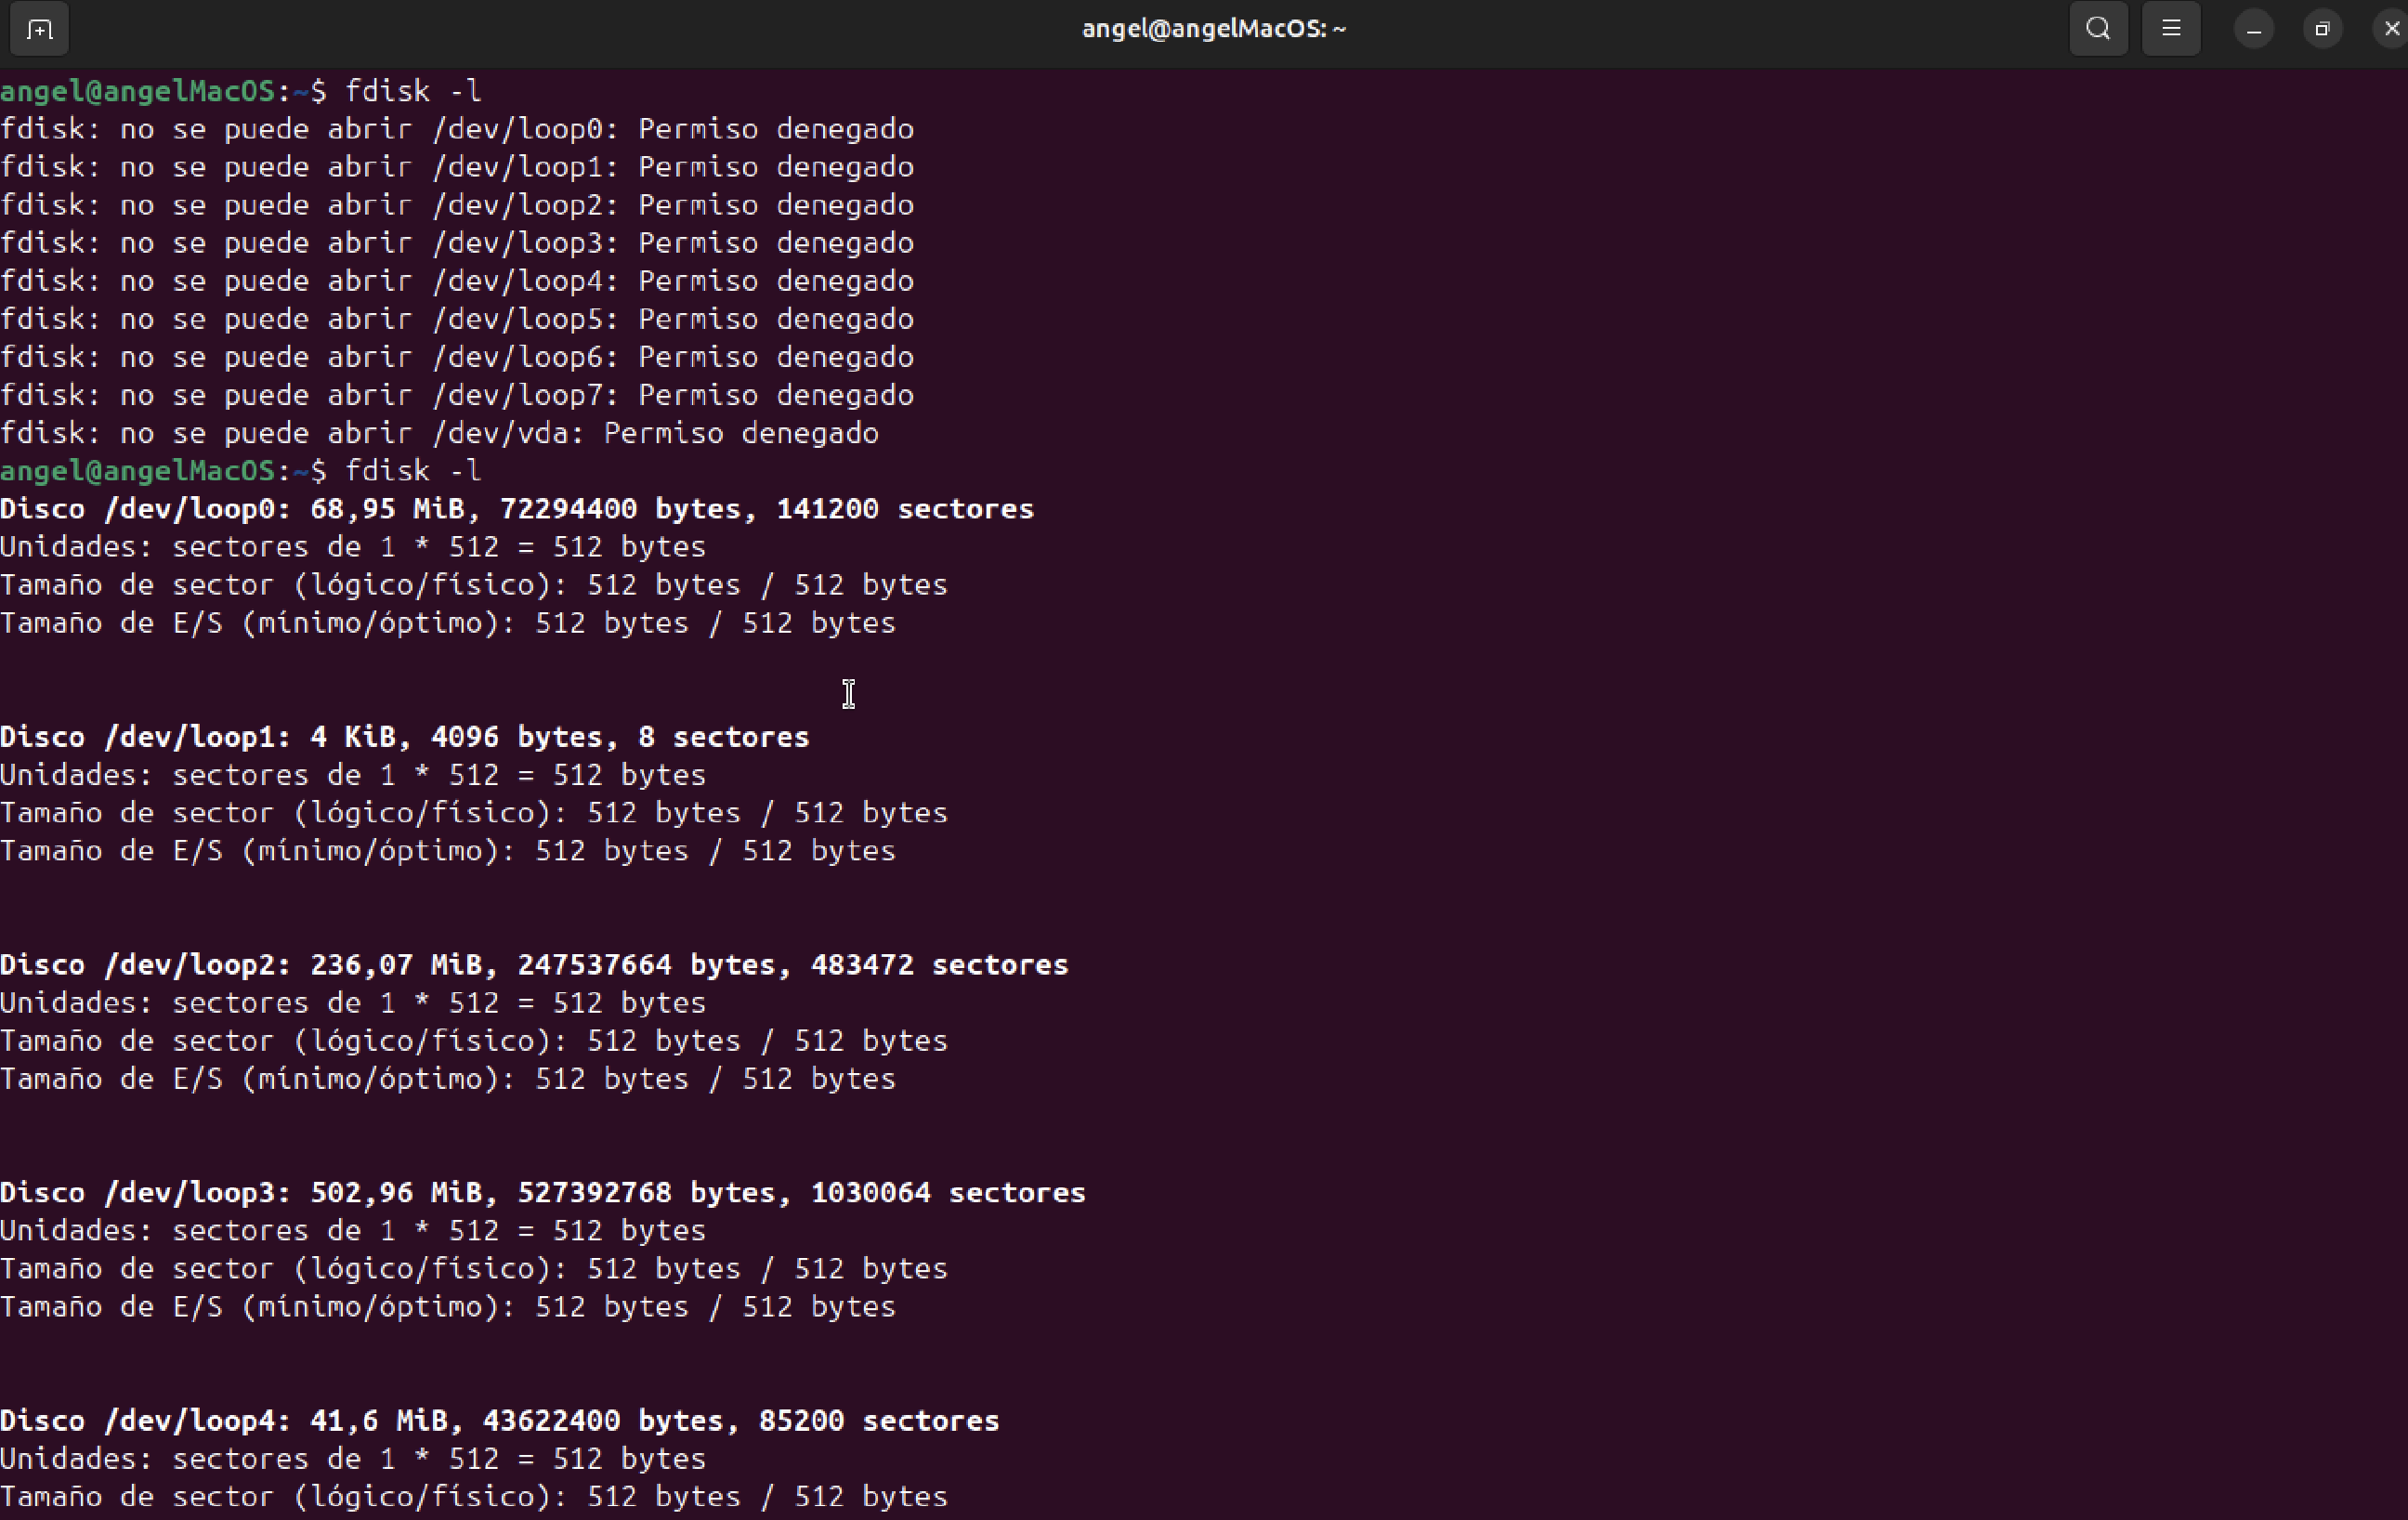
\includegraphics[width=0.6\textwidth]{image/image5.png}
    \caption{Ejecución del comando fdisk -l, para usuario no root, despues de activar el setuid.}
\end{figure}

\newpage

\subsection{Regreso de permisos originales:}

Por ultimo para poder regresar a los permisos originales que teniamos 
se tiene que ejecutar el comando \texttt{chmod 755 /sbin/fdisk}, esto es para poder regresar los permisos originales que teniamos, esto es debido a que el comando fdisk tiene acceso a la tabla de particiones del disco duro, y si un usuario sin permisos de administrador lo ejecuta, este no tendra acceso a la tabla de particiones y por lo tanto no podra ejecutar el comando.

\begin{figure}[H]
    \centering
    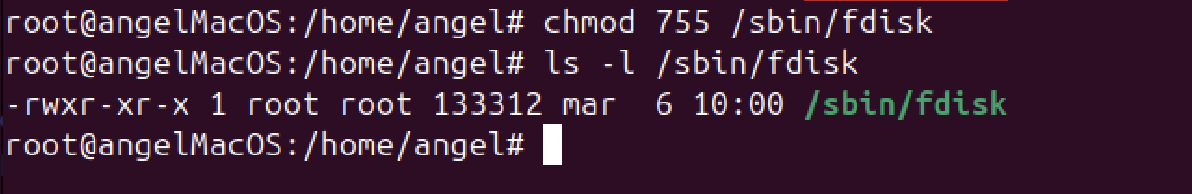
\includegraphics[width=0.7\textwidth]{image/image6.png}
    \caption{Ejecución del comando chmod para regresar los permisos originales.}
  
\end{figure}

\section{Actividad 2:}
Enunciado:
\textbf{Ahora haz que el programa sea de un usuario y trata de ejecutarlo como otro usuario. Modifica el bit “setuid” para que veas diferencia entre el usuario real y el usuario efectivo. }

El codigo para este caso es el del archivo \texttt{programa02\_ids.c}, donde en este codigo se obtienen los ids efectivos correspondientes, el id
del usuario real, el id del usuario efectivo, el id del grupo real y por ultimo 
el id del grupo efectivo, esto es para poder ver la diferencia entre el usuario real y el usuario efectivo.



Para poder ver primero quien tiene los derechos del archivo, 
se debe ejecutar el comando \texttt{ls -l programa02\_ids.c}.


Como se ve en la terminal de la derecha, el que tiene el derecho del archivo es ``angel'', donde este caso, ahora en la terminal de la izquierda 
que es la terminal siendo root, vamos a cambiar el dueño del archivo,
esto por medio del comando \texttt{chown root:root programa2}, ahora si en la terminal de la deerecha siendo la de angel, tratamos de correr el programa 
directamente nos mandara un error, esto debido a que el usuario angel no tiene los permisos para ejecutar el programa, esto es debido a que el dueño del archivo es root.

De hecho de igual forma comprobando con el comando \texttt{ls -l programa2}, vemos que ahora es root el dueño del programa.

\begin{figure}[H]
    \centering
    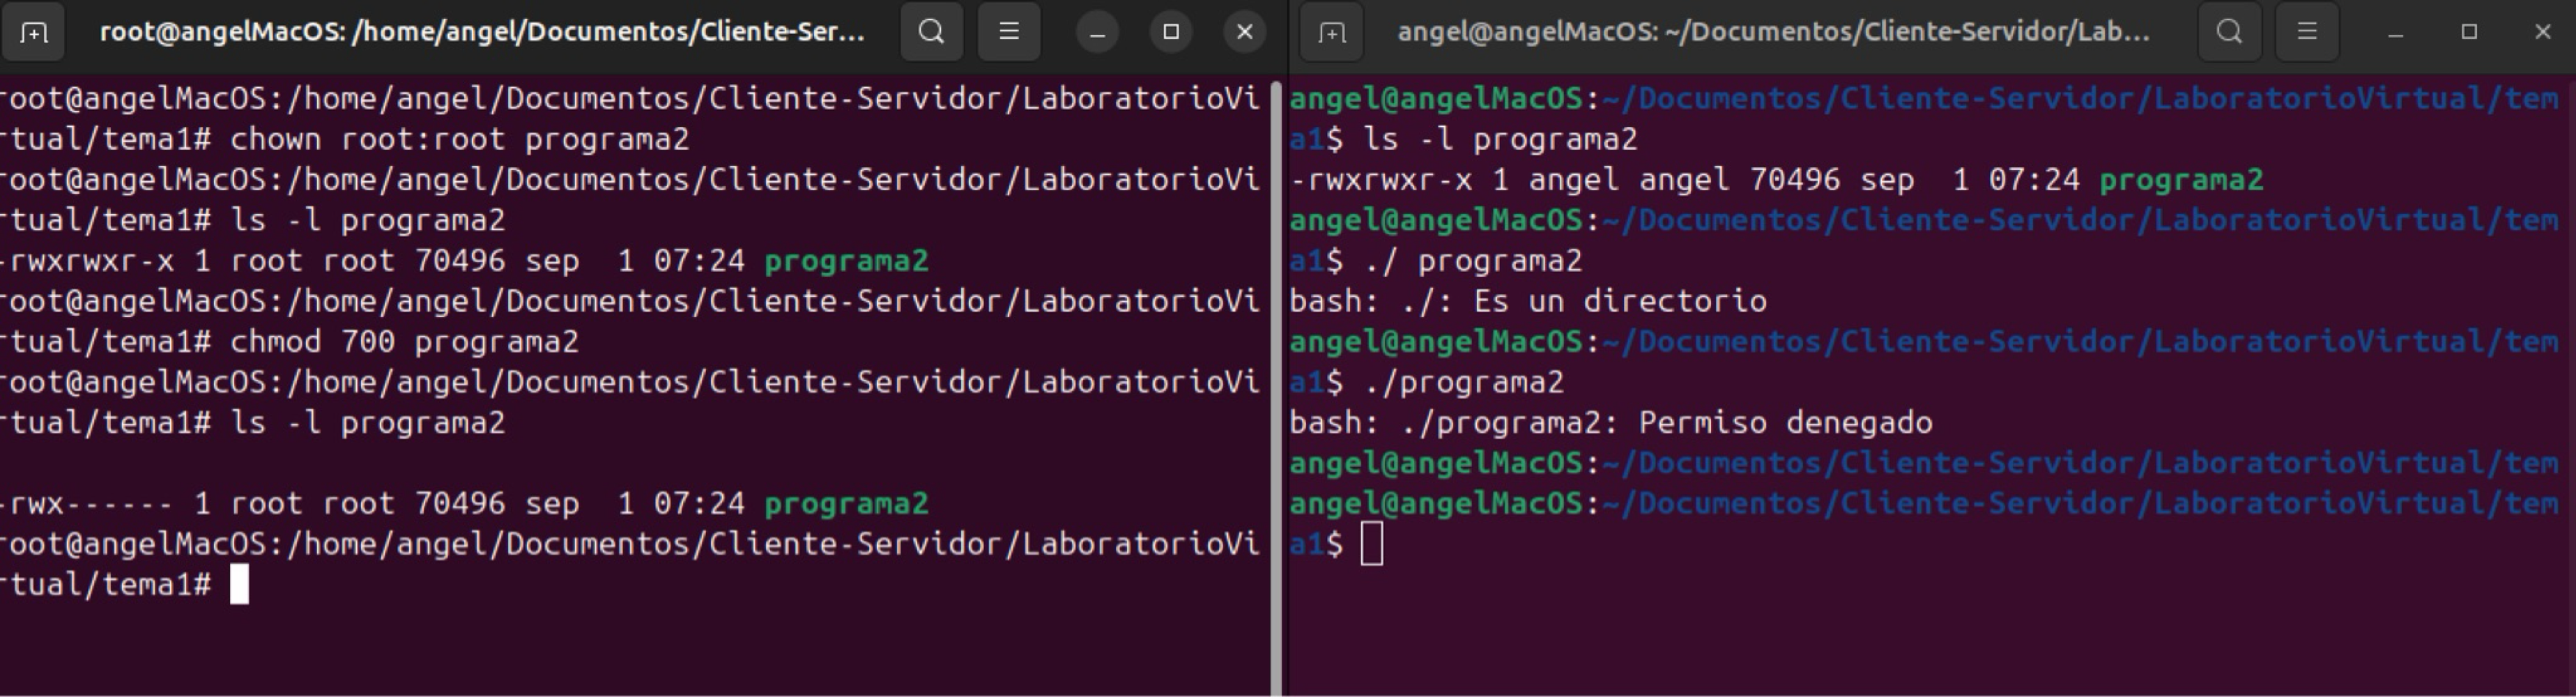
\includegraphics[width=1\textwidth]{image/image7.png}
    \caption{Ejecución del comando ls -l programa02, para ver los permisos del archivo.}
\end{figure}

Por ultimo ahora tenemos que activar el setuid, esto por medio del 
comando \texttt{chmod 4511 programa2}, esto es para que el programa pueda ser ejecutado por cualquier usuario.

\begin{figure}[H]
  \centering
  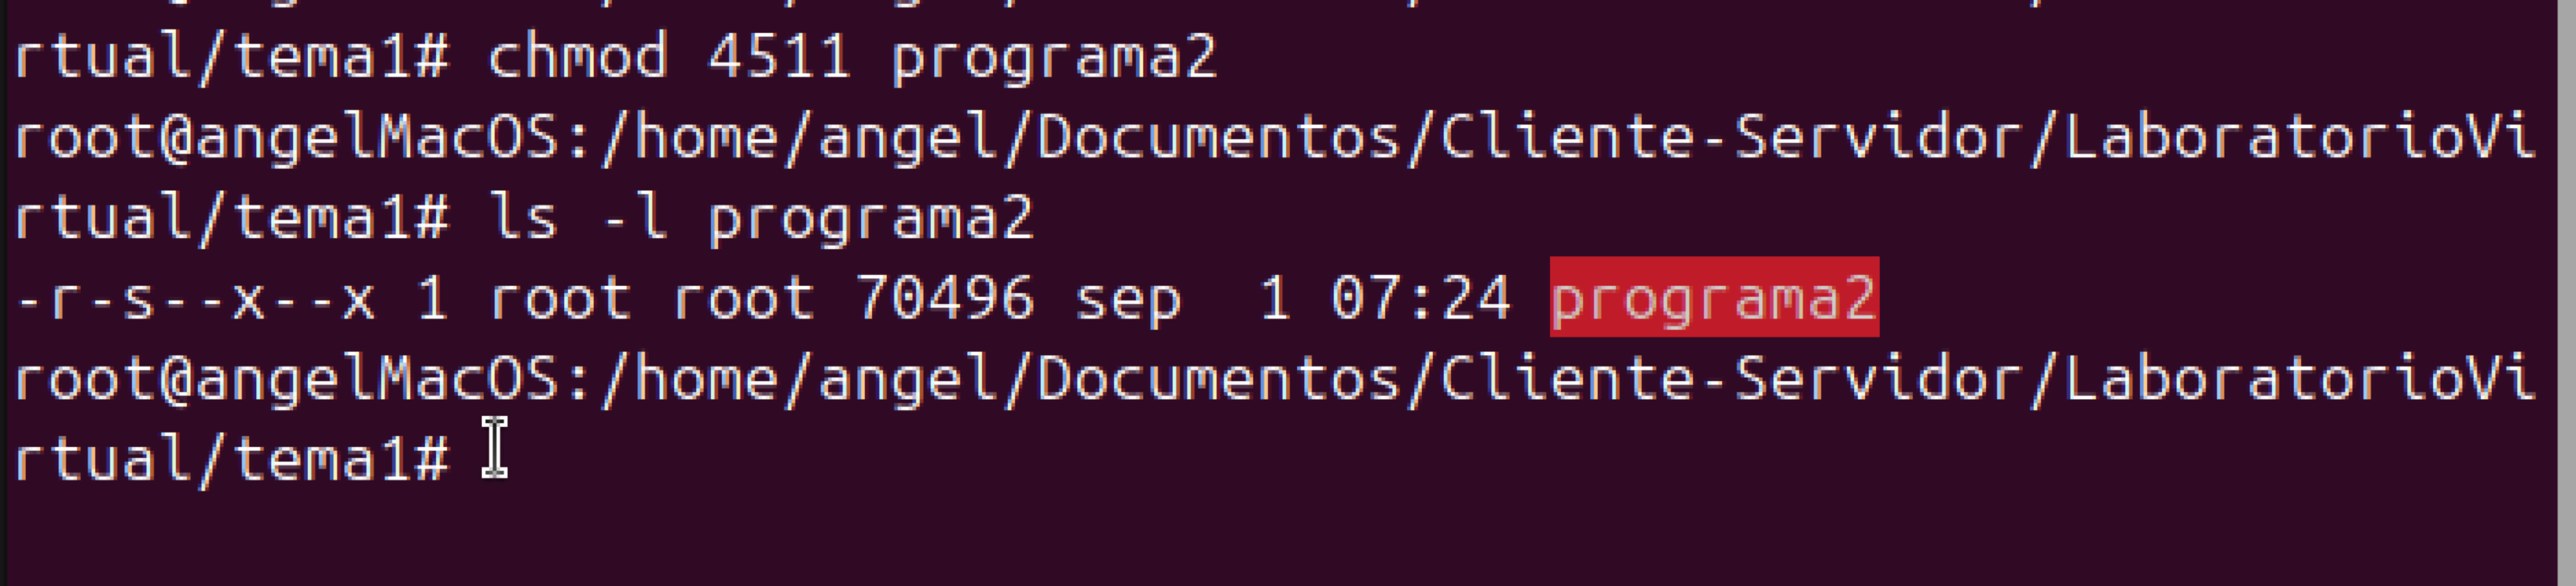
\includegraphics[width=1\textwidth]{image/image8.png}
  \caption{Ejecución del comando chmod para activar el setuid.}
\end{figure}

Con esto como se muestra en la terminal, ahora el id del usuario real y el 
id del usuario efectivo son diferentes, esto es debido a que el programa esta siendo ejecutado por un usuario diferente al que tiene los permisos del archivo, esto es debido a que el programa esta siendo ejecutado por el usuario angel, pero el programa tiene los permisos del usuario root, 
asi que durante la ejecucion del programa, este se vuelve root, y por lo tanto el id del usuario efectivo es diferente al id del usuario real.


\begin{figure}[H]
  \centering
  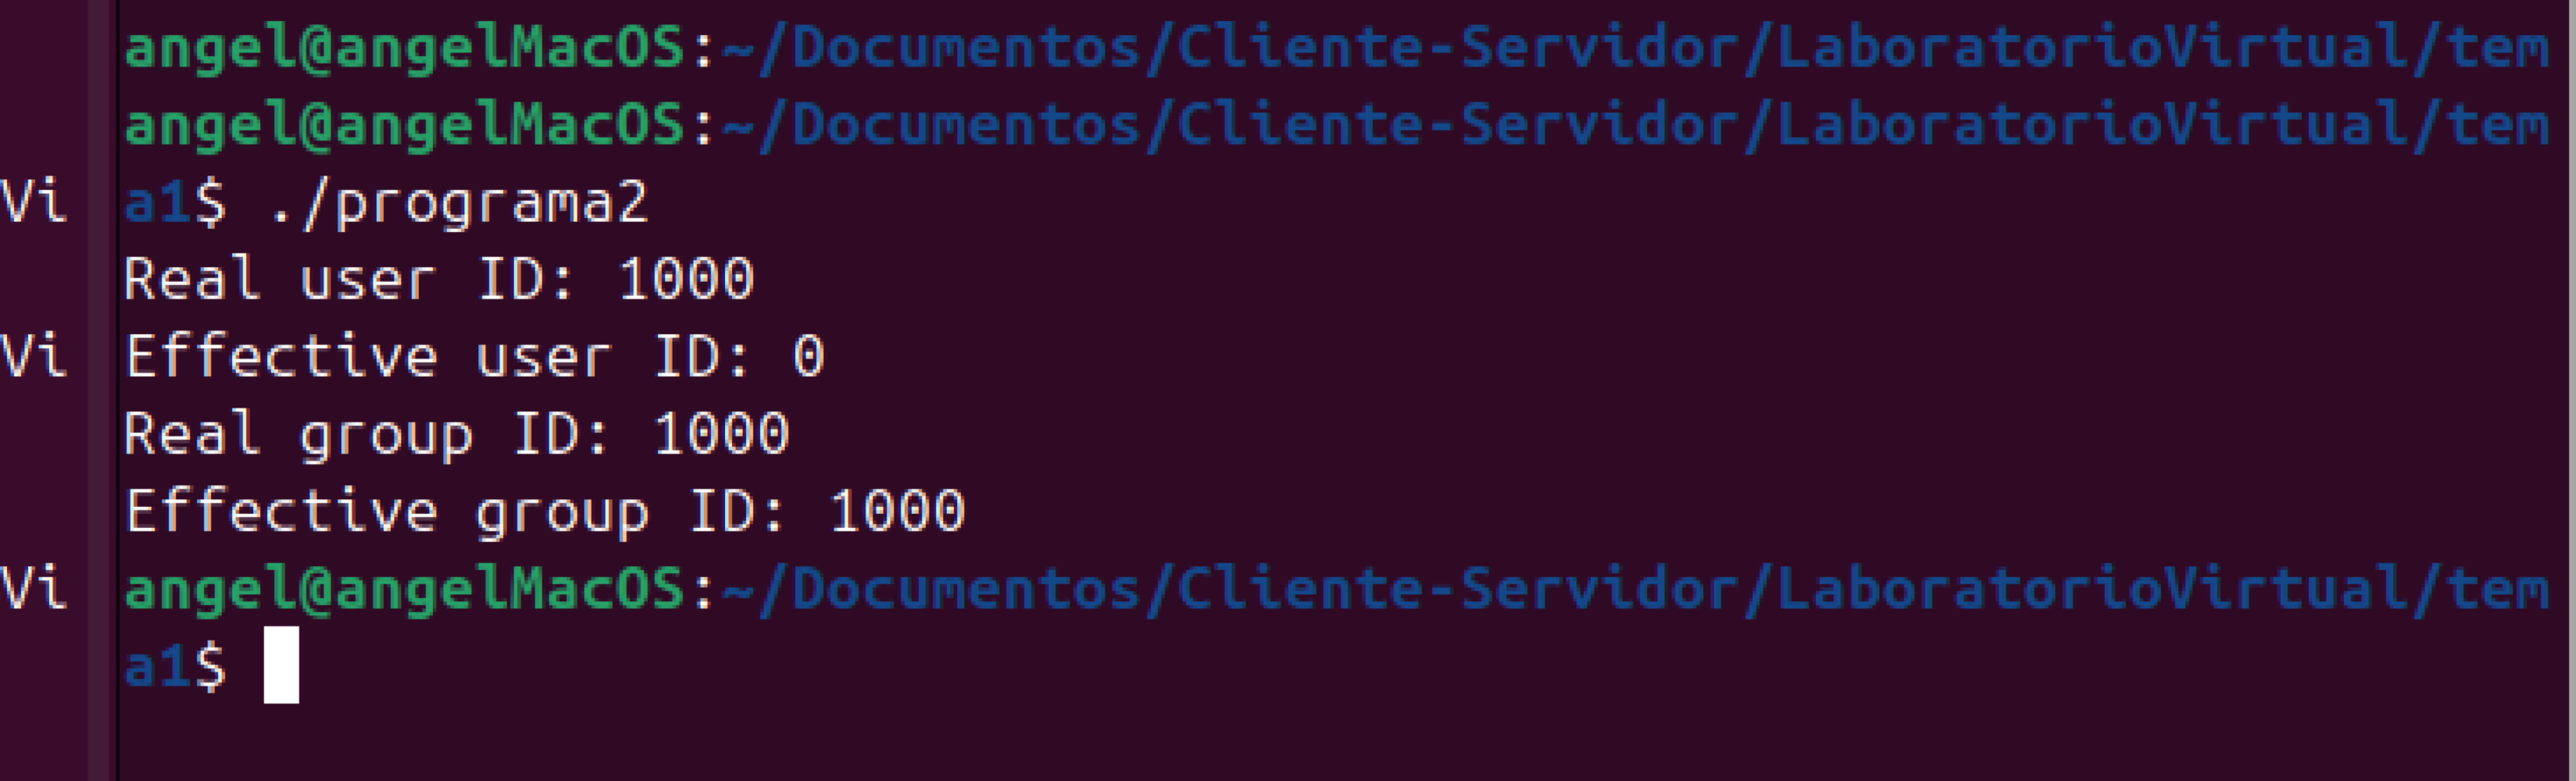
\includegraphics[width=1\textwidth]{image/image9.png}
  \caption{Ejecución del programa para ver la diferencia entre el usuario real y el usuario efectivo.}
  
\end{figure}


\thispagestyle{empty}

% Impresión Referencias
\nocite{*}
\printbibliography[heading=bibintoc, title={Referencias}]

\end{document}